%für Sprache, A4 Blatt, float, Grafiken, UTF Codierung, PDF, Color, Seitenabstand, Listings
\documentclass[a4papr,12pt]{article}
\usepackage[utf8]{inputenc}
\usepackage[ngerman]{babel}
\usepackage{graphicx}
\usepackage{float}
\usepackage{textcomp}
\usepackage{pdfpages}
\usepackage{tikz}
\usepackage{hyperref}
\usepackage{geometry}
\usepackage{listings}
\usepackage{color}
\usepackage{grffile}
\usepackage{caption}

%Mathematics
\usepackage{amstext}
\usepackage{amssymb}
\usepackage{amsmath}
\usepackage{amsfonts}
\usepackage{mathrsfs}
\usepackage{mathtools}

%include this before fancy or page style gets messed up bc of geometry
%Seitenabstand A4 Blatt
\geometry{a4paper}
\geometry{top=25mm,bottom=25mm,left=23mm,right=20mm}

% macro to select a scaled-down version of Bera Mono (for instance)
\makeatletter
\newcommand\BeraMonottfamily{%
  \def\fvm@Scale{0.85}% scales the font down
  \fontfamily{fvm}\selectfont% selects the Bera Mono font
}
\makeatother

%Hyperref zum anklicken von Überschriften in Texmaker + Farben einstellen
\hypersetup{
	colorlinks,
	citecolor=black,
	filecolor=black,
	linkcolor=blue,
	urlcolor=black
}

\definecolor{mygreen}{rgb}{0,0.6,0}
\definecolor{mygray}{rgb}{0.5,0.5,0.5}
\definecolor{mymauve}{rgb}{0.58,0,0.82}

%Zum Pascal Code einfügen mit lstinputlisting[language=Pascal] {../blabla.pas}
\lstset{ %
  backgroundcolor=\color{white},   % choose the background color; you must add \usepackage{color} or 								  \usepackage{xcolor}
  basicstyle=\BeraMonottfamily,        % the size of the fonts that are used for the code
  breakatwhitespace=false,         % sets if automatic breaks should only happen at whitespace
  breaklines=true,                 % sets automatic line breaking
  captionpos=b,                    % sets the caption-position to bottom
  commentstyle=\color{mygreen},    % comment style
  deletekeywords={...},            % if you want to delete keywords from the given language
  escapeinside={\%*}{*)},          % if you want to add LaTeX within your code
  extendedchars=true,              % lets you use non-ASCII characters; for 8-bits encodings only, 												does not work with UTF-8
  frame=single,	               % adds a frame around the code
  keepspaces=true,                 % keeps spaces in text, useful for keeping indentation of code 									  (possibly needs columns=flexible)
  keywordstyle=\color{blue},       % keyword style
  language=Octave,                 % the language of the code
  otherkeywords={...},           % if you want to add more keywords to the set
  numbers=left,                    % where to put the line-numbers; possible values are (none, left, 								  right)
  numbersep=5pt,                   % how far the line-numbers are from the code
  numberstyle=\tiny\color{black}, % the style that is used for the line-numbers
  rulecolor=\color{black},         % if not set, the frame-color may be changed on line-breaks within 								  not-black text (e.g. comments (green here))
  showspaces=false,                % show spaces everywhere adding particular underscores; it 														overrides 'showstringspaces'
  showstringspaces=false,          % underline spaces within strings only
  showtabs=false,                  % show tabs within strings adding particular underscores
  stepnumber=2,                    % the step between two line-numbers. If it's 1, each line will be 								  numbered
  stringstyle=\color{mymauve},     % string literal style
  title=\getlstname,
  tabsize=2,	                    % sets default tabsize to 2 spaces
  inputencoding=latin1,
  columns=fullflexible
}

\lstset{literate=%
	{Ö}{{\"O}}1
	{Ä}{{\"A}}1
	{Ü}{{\"U}}1
	{ß}{{\ss}}1
	{ü}{{\"u}}1
	{ä}{{\"a}}1
	{ö}{{\"o}}1
	{~}{{\textasciitilde}}1
}

%Filenamen und Pfad trennen
\makeatletter
\DeclareRobustCommand{\getlstname}{%
\begingroup
  % \lstname seems to change hyphens into \textendash
  \def\textendash{-}%
  \filename@parse{\lstname}%
  \texttt{\filename@base.\filename@ext}%
\endgroup
}


%Für Kopfzeile den Style
\usepackage{fancyhdr}
\pagestyle{fancy}
\lhead{AUD 2\textbackslash PRO 2 - Übung 5}
\rhead{Andreas Roither, \today{}}
\newcommand{\Cross}{\mathbin{\tikz [x=1.4ex,y=1.4ex,line width=.2ex] \draw (0,0) -- (1,1) (0,1) -- (1,0);}}%

\begin{document}

%ANGABE     
\thispagestyle{plain}
\includepdf[pages={1},pagecommand={     
\begin{tikzpicture}[remember picture, overlay]\node at (15.8, -0.85) {6 h};\end{tikzpicture}
\begin{tikzpicture}[remember picture, overlay]\node at (7.6, -0.85) {Andreas Roither};\end{tikzpicture}
\begin{Huge}
\begin{tikzpicture}[remember picture, overlay]\node at (-1.3, -1.9) {X};\end{tikzpicture}
\end{Huge}
}]{Angabe/UE5.pdf}
%\thispagestyle{plain}
%\includepdf[pages=2-,pagecommand={}]{Angabe/UE4.pdf}

\section*{Übung 5}
\subsection*{Aufgabe 1}
\subsubsection*{Lösungsidee}
Es wird eine ATG für Infix zu Prefix erstellt. Mithilfe dieser ATG wird ein entsprechende Implementation vorgenommen.  Um eine Prefix-Notation zu erreichen wird Auf oberster Ebene ( Expr ) alles aus den unteren Ebene ( bzw. aus den Aufrufen von Term und Fact ) aneinander gehängt. Somit wird eine Prefix-Notation erreicht.  
\newline
\lstinputlisting[language=] {../InfixToPrefixATG.txt}
Die ATG für Infix zu Prefix.
\newpage
\lstinputlisting[language=Pascal] {../InfixToPrefix.pas}
\begin{figure}[H]
	\centering
	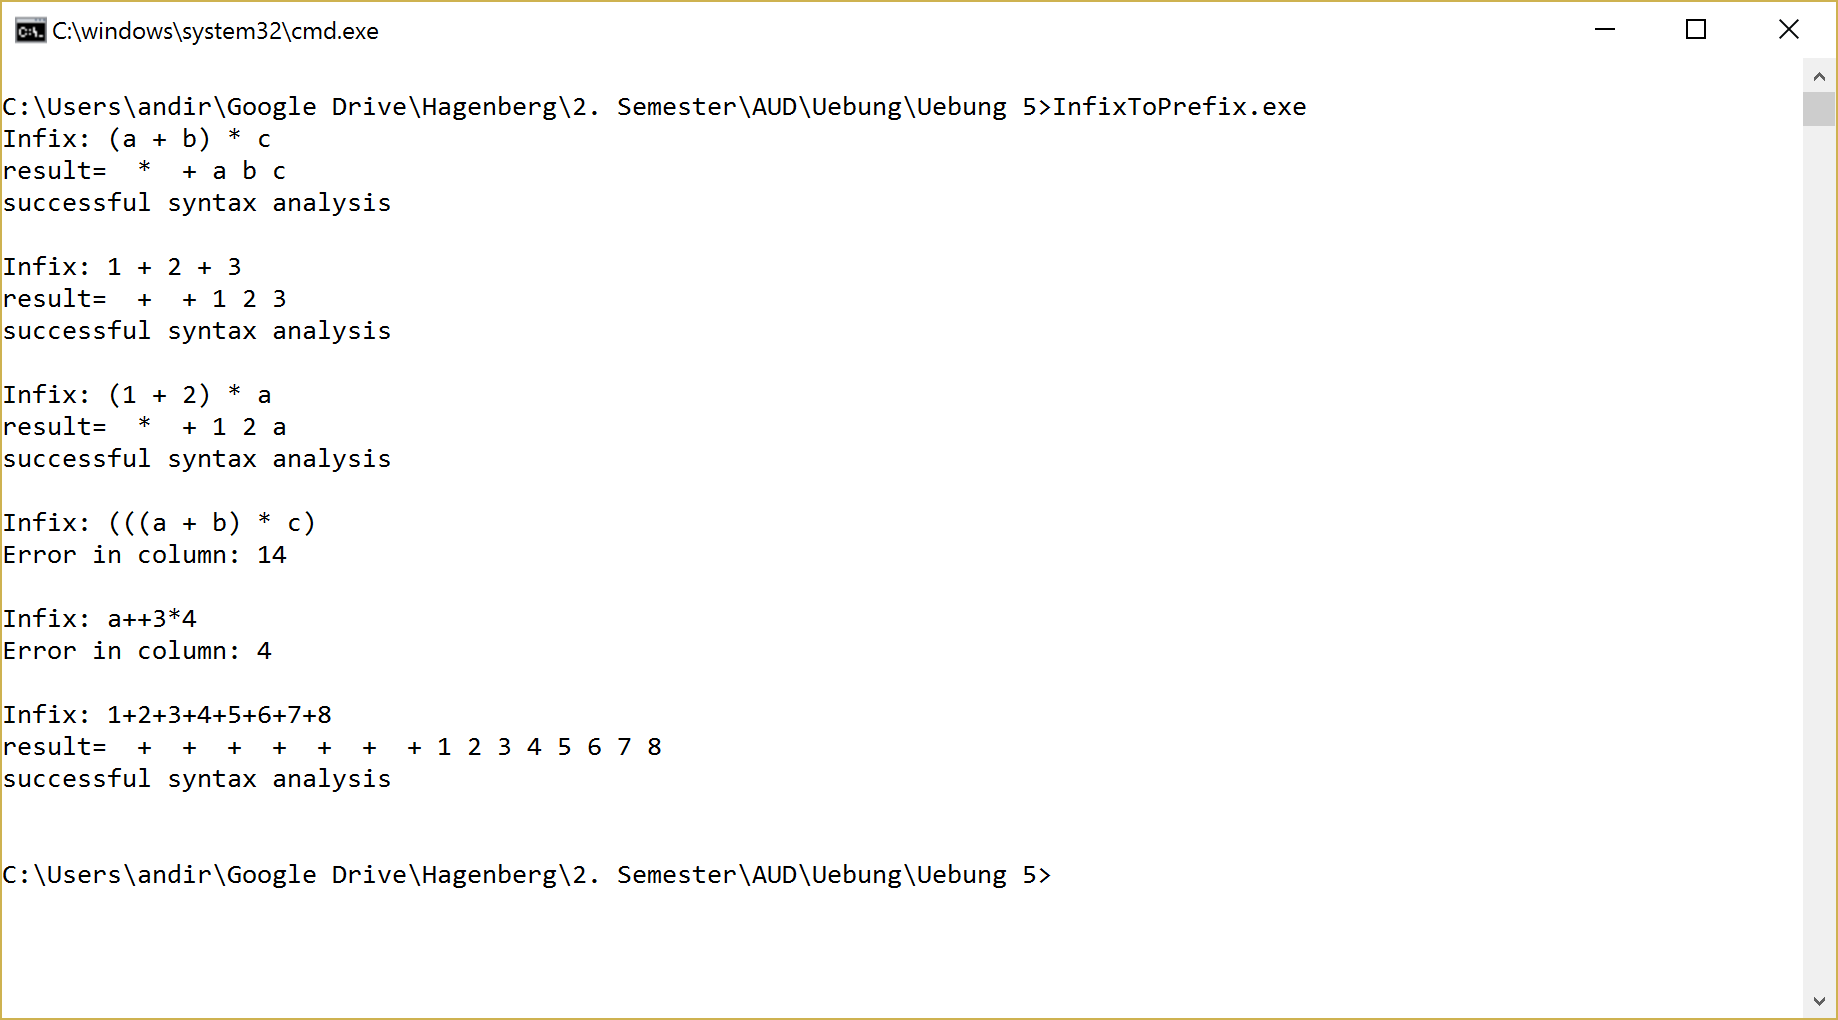
\includegraphics[scale=0.7]{./pictures/1.png}
	\caption{Infix to Prefix Test }
	\label{fig: InfixToPrefix}
\end{figure}
\raggedright
Die Testfälle zeigen sowohl funktionierende Testfälle als auch Testfälle mit eingebauten Fehlern. Falls zu viele Klammern oder Rechenoperationszeichen übergeben werden, wird eine Fehler Meldung ausgegeben. Die Spalten Nummer bei der Fehler Meldung funktioniert dabei leider nicht immer. Result zeigt die Prefix-Notation.

\newpage
\subsection*{Aufgabe 2}
\subsubsection*{Lösungsidee}
Die ATG funktioniert ähnlich wie bei Aufgabe 1. Der Unterschied besteht darin das der Baum ohne eine Insert Funktion aufgebaut wird. Die Nodes werden aneinander gehängt und somit wird der Baum aufgebaut. Auf oberster Ebene ( oberster Funktionsaufruf, oder erste Funktion die aufgerufen wird von Expr, Term, Fact ) wird eine Node mit den anderen Nodes aus den Funktionsaufruf Term aneinander gehängt. Bei \grqq{}1 + 2\grqq{} wäre f1 eine Node mit \grqq{}1\grqq{} in txt und f2 eine Node mit \grqq{}2\grqq{} in txt gespeichert. Mit diesen Nodes wird eine neue Node erstellt, mit \grqq{}+\grqq{} als Wurzelknoten und f1, f2 als die beiden sub trees. Die anderen Funktionen geben immer eine Node zurück, entweder mit einem \grqq{}+\grqq{}, \grqq{}-\grqq{} oder einer Zahl als Wurzelknoten. Die rekursive Funktion wird mithilfe eines case statements implementiert. Je nachdem welches Zeichen in der aktuellen Node enthalten ist wird eine der vier Rechenoperationen ausgeführt. Bei den verschiedene Ausgaben InOrder, PreOrder, PostOrder fällt auf das InOrder den Baum ähnlich ausgibt wie den ursprünglichen Input nur ohne Klammern, PreOrder gibt den Baum aus wie Prefix-Notation und PostOrder wie Postfix-Notation.
\newline

\lstinputlisting[language=] {../TreeATG.txt}
\newpage
\lstinputlisting[language=Pascal] {../TreeEval.pas}
\begin{figure}[H]
	\centering
	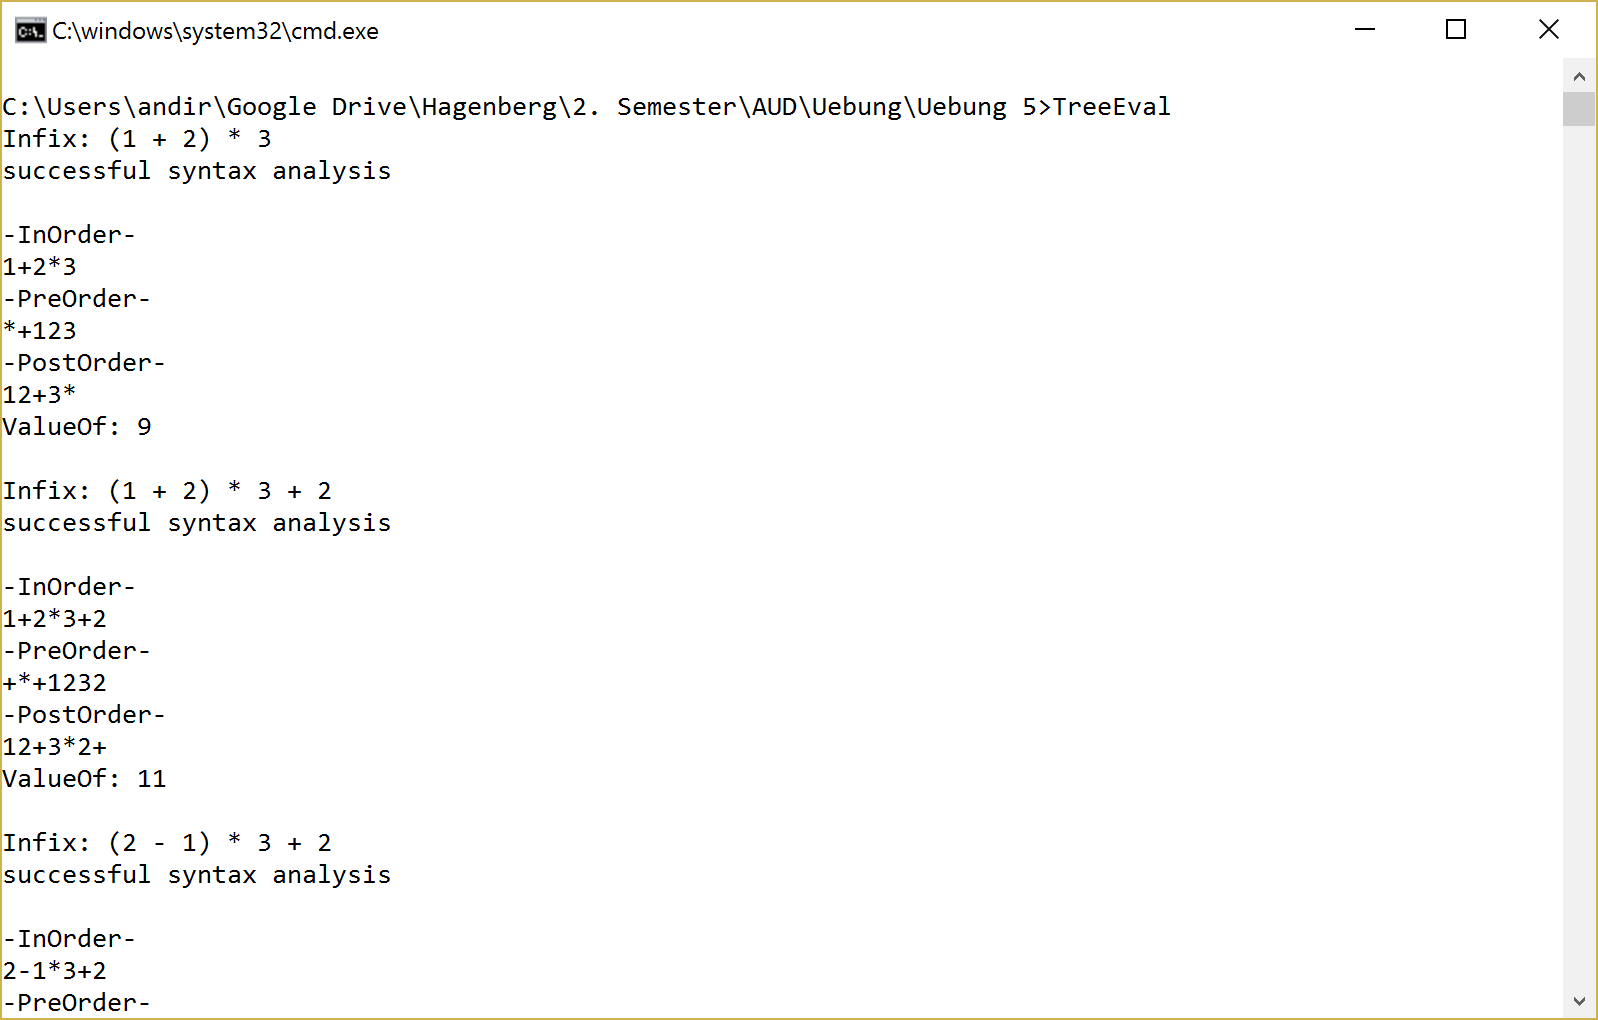
\includegraphics[scale=0.8]{./pictures/2_1.png}
	\caption{TreeEval Test 1}
	\label{fig: Matching}
\end{figure}
\begin{figure}[H]
	\centering
	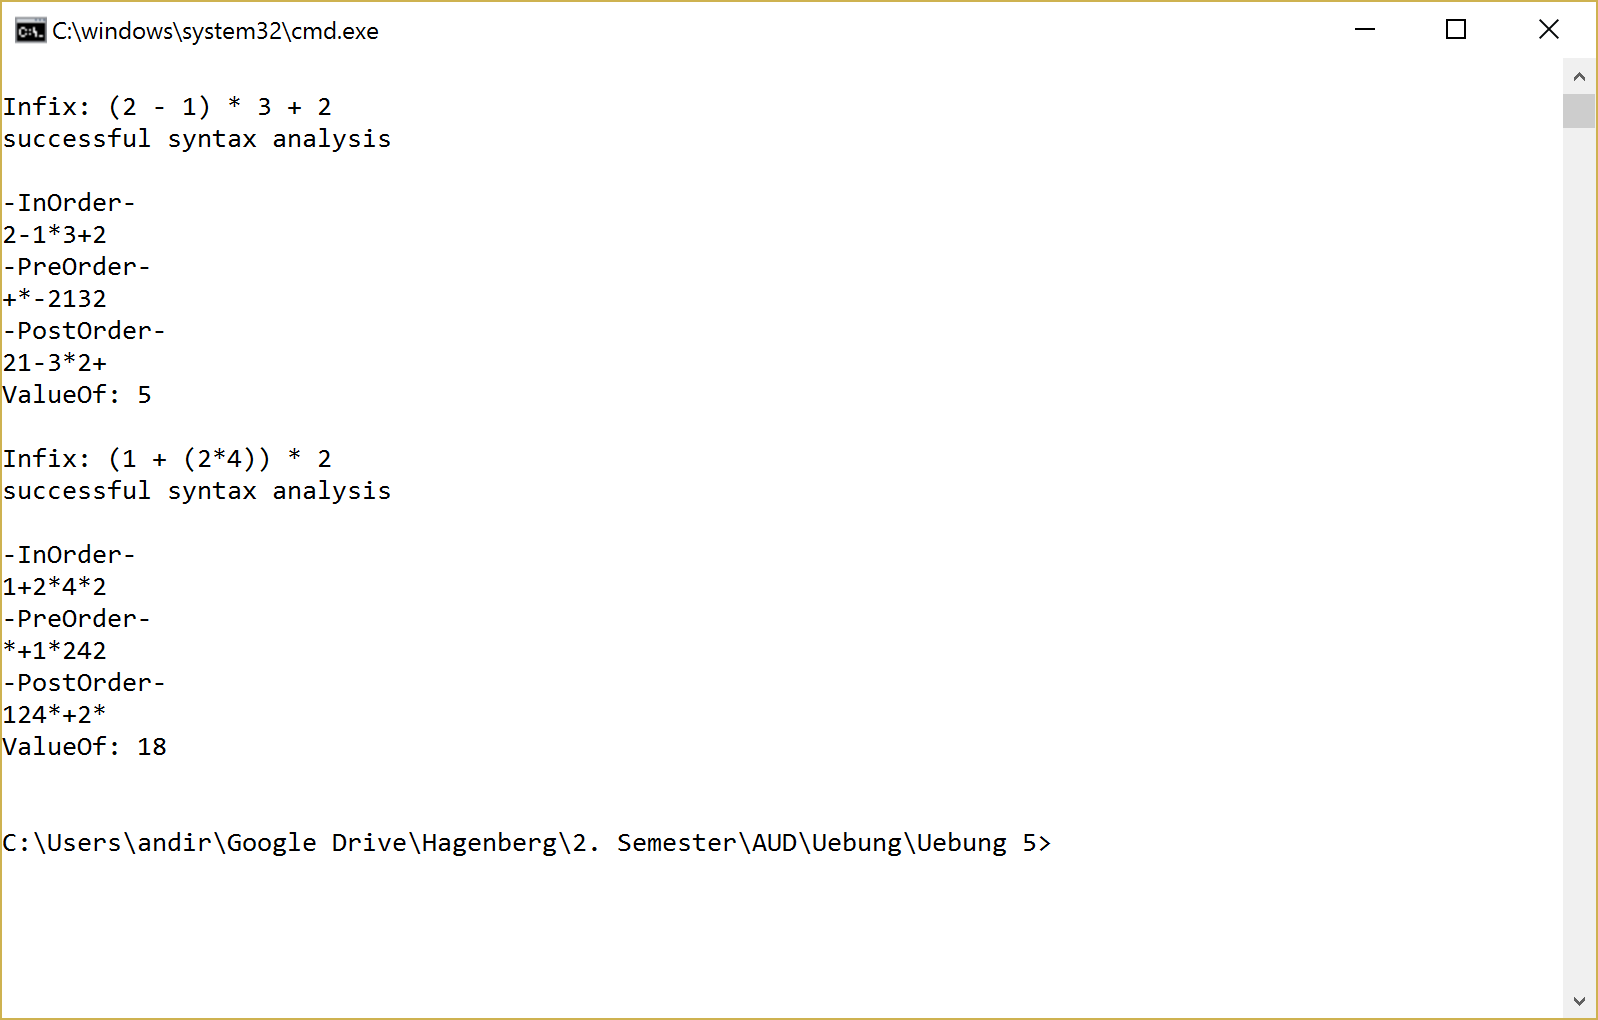
\includegraphics[scale=0.8]{./pictures/2_2.png}
	\caption{TreeEval Test 2}
	\label{fig: Matching}
\end{figure}
\raggedright
Die verschiedene Testfälle zeigen die Syntax Analysis, InOrder, PreOrder, PostOrder Ausgabe des Baumes und das verwenden der ValueOf Funktion. Die ValueOf Funktion führt alle Rechenoperationen im Baum aus und liefert das ausgerechnete Ergebnis zurück.
\newpage


\end{document}





